
% v2-acmsmall-sample.tex, dated March 6 2012
% This is a sample file for ACM small trim journals
%
% Compilation using 'acmsmall.cls' - version 1.3 (March 2012), Aptara Inc.
% (c) 2010 Association for Computing Machinery (ACM)
%
% Questions/Suggestions/Feedback should be addressed to => "acmtexsupport@aptaracorp.com".
% Users can also go through the FAQs available on the journal's submission webpage.
%
% Steps to compile: latex, bibtex, latex latex
%
% For tracking purposes => this is v1.3 - March 2012
\documentclass[prodmode,acmtecs]{acmsmall} % Aptara syntax
\usepackage[spanish,polish]{babel}
\usepackage[T1]{fontenc}
\usepackage{fancyvrb}
\usepackage{graphicx,hyperref}
\newcommand\cutout[1]{}


\usepackage[table]{xcolor}
\usepackage[utf8]{inputenc}
\usepackage[parfill]{parskip}
\usepackage{tabulary}
\PassOptionsToPackage{hyphens}{url}
\usepackage{hyperref}    
\usepackage[capitalize]{cleveref}


% Metadata Information
% !!! TODO: SET THESE VALUES !!!
\acmVolume{0}
\acmNumber{0}
\acmArticle{CFP}
\acmYear{0}
\acmMonth{0}

\newcounter{colstart}
\setcounter{page}{4}

\RecustomVerbatimCommand{\VerbatimInput}{VerbatimInput}%
{
%fontsize=\footnotesize,
fontfamily=\rmdefault
}


\newcommand{\UnderscoreCommands}{%\do\verbatiminput%
\do\citeNP \do\citeA \do\citeANP \do\citeN \do\shortcite%
\do\shortciteNP \do\shortciteA \do\shortciteANP \do\shortciteN%
\do\citeyear \do\citeyearNP%
}

\usepackage[strings]{underscore}



% Document starts
\begin{document}


\setcounter{colstart}{\thepage}

\acmArticle{CFP}
\title{{\huge\sc SIGLOG Monthly 239}

 July 2023}
\author{DAVID PURSER\affil{University of Liverpool, UK}
\vspace*{-2.6cm}\begin{flushright}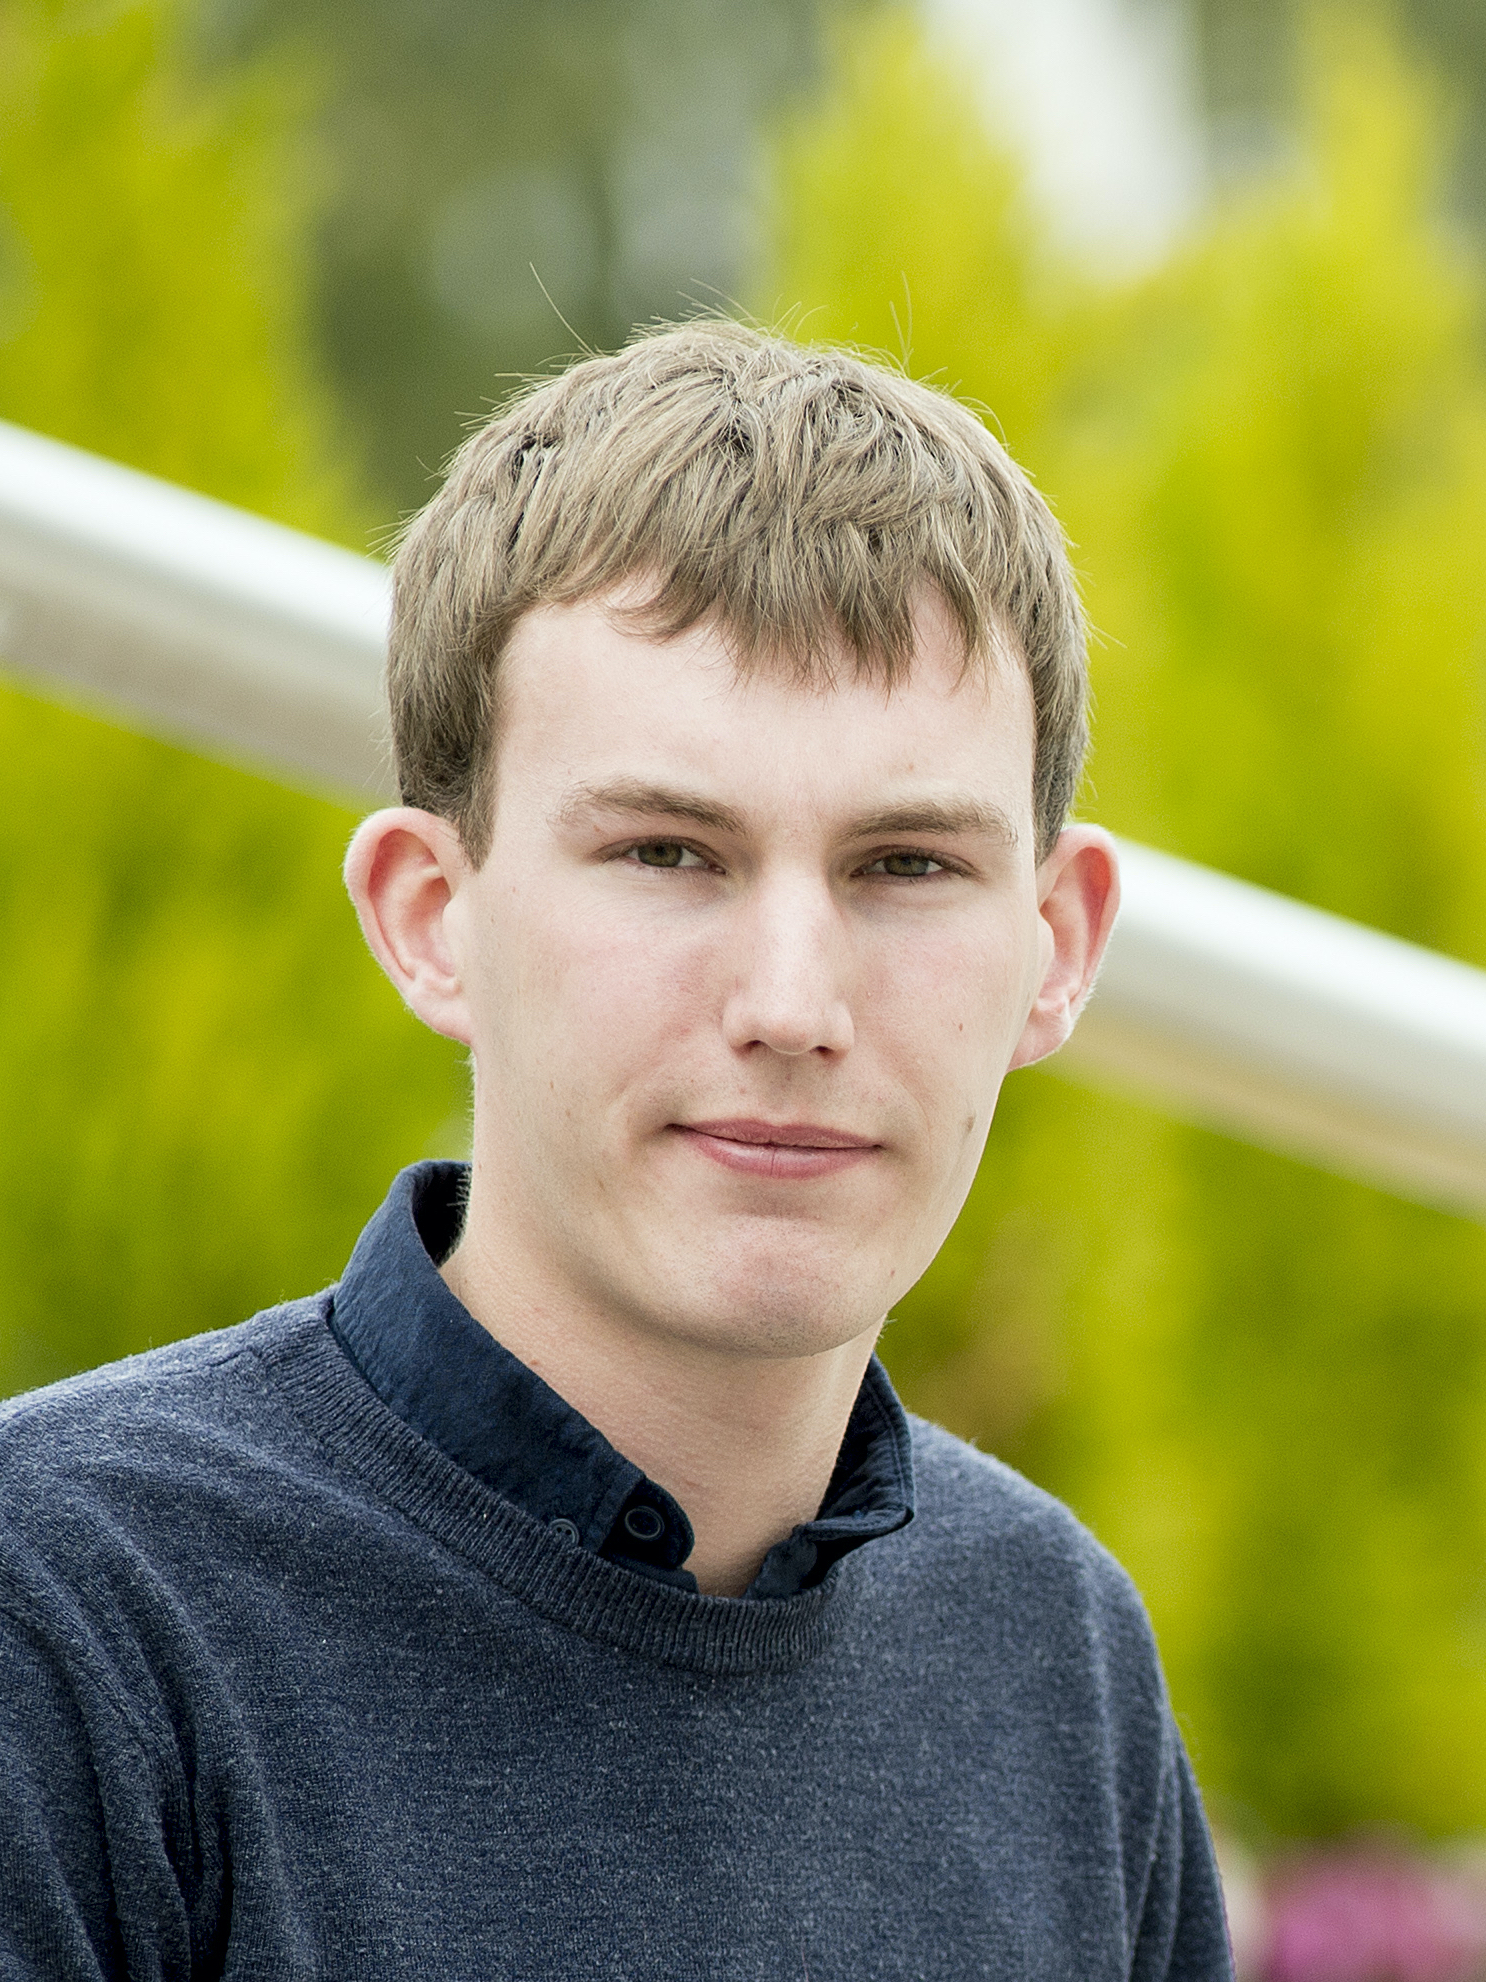
\includegraphics[width=30mm]{dp}\end{flushright}
}

\begin{abstract}
July 2023 edition of SIGLOG Monthly, featuring deadlines, calls and community announcements.
\end{abstract}


\maketitlee

\href{https://lics.siglog.org/newsletters/}{Past Issues}
 - 
\href{https://lics.siglog.org/newsletters/inst.html}{How to submit an announcement}
\section{Table of Content}\begin{itemize}\item DEADLINES (\cref{deadlines}) 
 
\item CALLS 
 
\begin{itemize}\item IFIP WG 1.6 (CALL FOR PARTICIPATION) (\cref{IFIPWG16})
\item EUMAS PhD Day 2023 (CALL FOR CONTRIBUTIONS) (\cref{EUMASPhDDay2023})
\item STAF 2023 (CALL FOR PARTICIPATION) (\cref{STAF2023})
\item ICGT 2023 (CALL FOR PARTICIPATION) (\cref{ICGT2023})
\item RSSRail 2023 (CALL FOR POSTERS) (\cref{RSSRail2023})
\item Infinity 2023 (CALL FOR CONTRIBUTIONS AND PARTICIPATION) (\cref{Infinity2023})
\end{itemize} 
\end{itemize}\section{Deadlines}\label{deadlines}\rowcolors{1}{white}{gray!25}\begin{tabulary}{\linewidth}{LL}PhD or Postdoc position at KIT in Logic of Autonomous Dynamical Systems:  & Jul 03, 2023 (Application deadline) \\
EUMAS PhD Day 2023:  & Jul 08, 2023 (Paper Submission Deadline) \\
RSSRail 2023:  & Jul 14, 2023 (Poster) \\
CSL'24:  & Jul 24, 2023 (Abstract), Jul 31, 2023 (Paper) \\
RW 2023:  & Aug 10, 2023 (Application deadline) \\
Infinity 2023:  & Aug 15, 2023 (Talk) \\
Postoctoral Positions Augusta University (Georgia, USA):  & Sep, 2023 (preferably or until filled) \\
ICDT 2024:  & Sep 13, 2023 (Cycle 2 Abstract), Sep 20, 2023 (Cycle 2 Full) \\
\end{tabulary}
\section{IFIP WG 1.6: Meeting of the IFIP Working Group 1.6 on Rewriting}\label{IFIPWG16}  5 July 2023\\ 
  Rome, Italy\\ 
  \href{https://ifip-wg-rewriting.cs.ru.nl/events/event-2023.html}{https://ifip-wg-rewriting.cs.ru.nl/events/event-2023.html}\\ 
CALL FOR PARTICIPATION 

\begin{itemize}\item  Both members and non-members of the working group are invited to attend the public section of the upcoming meeting of the IFIP Working Group 1.6 on Rewriting (IFIP WG 1.6) 
 
\item  REGISTRATION 
 
  The registration page for FSCD 2023 and affiliated events, such as the meeting of the IFIP WG 1.6, is available here: 
 
  \href{https://easyconferences.eu/fscd2023/registration1/}{https://easyconferences.eu/fscd2023/registration1/} 
 
  Please note that FSCD participants still need to separately register for IFIP (but there is a discount). 
 
  Attending the meeting of the IFIP WG 1.6 is possible both in-person and remotely. All parts of the programme are public, except for the members-only business meeting at the end of the programme. 
 
\item  PROGRAM 
 
  See \href{https://ifip-wg-rewriting.cs.ru.nl/events/event-2023.html}{https://ifip-wg-rewriting.cs.ru.nl/events/event-2023.html} 
 
\item  More information about IFIP WG 1.6: 
 
  \href{https://ifip-wg-rewriting.cs.ru.nl/}{https://ifip-wg-rewriting.cs.ru.nl/} 
 
\end{itemize}\section{EUMAS PhD Day 2023: The 20th European Conference on Multi-Agent Systems PhD Day}\label{EUMASPhDDay2023}  12th and/or 13th September 2023 (exact day to be announced) University of Naples Federico II Naples, Italy\\ 
  Website: \href{https://vadimmalvone.github.io/eumas2023/}{https://vadimmalvone.github.io/eumas2023/} \\ 
  Contact: angelo.ferrando@unige.it, munyque.mittelmann@unina.it\\ 
CALL FOR CONTRIBUTIONS 

\begin{itemize}\item  IMPORTANT DATES 
 
\rowcolors{1}{white}{gray!25}\begin{tabulary}{\linewidth}{LL}Paper Submission Deadline:  & Jul 08, 2023 \\
Paper Notification:  & Jul 23, 2023 \\
Camera Ready:  & Jul 30, 2023 \\
\end{tabulary}
 
\item  SCOPE 
 
  EUMAS 2023 is an EURAMAS designated and aims to encourage and support activity in the research and development of multi-agent systems, in academic and industrial effort. The conference aspires to be the primary European forum for researchers interested in the theory and practice of autonomous agents and multi-agent systems. EUMAS enables researchers to meet, present challenges, preliminary and mature research results in an open environment. EUMAS 2023 features formal proceedings published as part of the Lecture Notes in Computer Science (LNCS) series of Springer 
 
  Phd Students (and also former PhD students that completed their PhD in 2022 or 2023) are invited to submit an Extended Abstract to EUMAS 2023. The accepted abstracts will be be presented during the EUMAS 2023 PhD Day (which will be held on the 12th or 13th of September, exact day TBA), and will be included in EUMAS 2023 proceedings. 
 
  All PhD day authors will give an highlight talk of their work (in 5 minutes) and then present it as a poster. There will be a best presentation award (based on the talk and the poster), which will come with a monetary prize. 
 
\item  Topics of interest include, but are not limited to: 
 
   Action and Planning; Adaptation and Learning; Agent Architectures; Agent Programming Languages; Agent Development Methodologies and Tools; Agent-Based Simulation; Agent Organizations and Institutions; Agent-oriented Software Engineering; Agents and Complex Systems; Applications of Multi-agent Systems; Argumentation; Automated negotiation; Biologically inspired approaches; Cognitive Models; Collective and Swarm Intelligence; Collective Intentionality; Communication, Cooperation, and Coordination - Computational Social Choice; Economic Models; Electronic Commerce; Ethical behavior of multi-agent systems; Formal Modelling; Game-Theoretic Methods - Human-Agent Interaction; Logics for Multi-Agent Systems; Logics for Strategic Reasoning; Negotiation; Self-organization; Semantic Web Agents - Social Networks; Socio-technical Systems; Theories of Agency; Trust and Reputation; Verification; Virtual Agents; Voting and Judgment Aggregation Models for multi-agent systems 
 
  All submissions will be peer-reviewed in a single blind fashion. Specifically, all submissions should not be anonymized. Submission should be at most 3 pages long, with 1 additional page only for references, and be formatted according to Springer’s LNCS format. For templates and instructions for authors, see \href{https://www.springer.com/gp/computer-science/lncs/conference-proceedings-guidelines}{https://www.springer.com/gp/computer-science/lncs/conference-proceedings-guidelines}. 
 
  Authors must submit their contributions through Easychair as a single PDF file: \href{https://easychair.org/conferences/?conf=eumas2023}{https://easychair.org/conferences/?conf=eumas2023}   
 
\end{itemize}\section{STAF 2023: Software Technologies: Applications and Foundations}\label{STAF2023}  July 18-21, 2023, Leicester, UK\\ 
  \href{https://conf.researchr.org/home/staf-2023}{https://conf.researchr.org/home/staf-2023}\\ 
CALL FOR PARTICIPATION 

\begin{itemize}\item  REGISTRATION INFORMATION:  
 
  \href{https://conf.researchr.org/attending/staf-2023/registration}{https://conf.researchr.org/attending/staf-2023/registration} 
 
\item  DRAFT PROGRAMME:  
 
  \href{https://conf.researchr.org/program/staf-2023/program-staf-2023/}{https://conf.researchr.org/program/staf-2023/program-staf-2023/} 
 
\item  ABOUT  
 
  Software Technologies: Applications and Foundations (STAF) is a federation of leading conferences on software technologies. It was formed after the end of the successful TOOLS federated event in 2012, providing a loose umbrella organisation with a steering committee that aims to provide continuity. The STAF federated event runs annually. The conferences that participate may vary from year to year, but all focus on practical and foundational advances in software technology. The conferences address all aspects of software technology, from object-oriented design, testing, mathematical approaches to modelling and verification, transformation, model-driven engineering, aspect-oriented techniques, and tools. 
 
  We invite you to join us at STAF 2023 in Leicester, UK from July 18-21, 2023! 
 
\item  KEYNOTE SPEAKERS 
 
\begin{itemize}\item  Kim G. Larsen, Aalborg University (Denmark)
\item  Dan Ghica, Huawei Research and University of Birmingham (UK)
\item  Mohammad Abdulaziz, King’s College London (UK)
\item  Andrzej Wąsowski, IT University of Copenhagen (Denmark)
\end{itemize} 
  More details: \href{https://conf.researchr.org/track/staf-2023/staf-2023-keynotes}{https://conf.researchr.org/track/staf-2023/staf-2023-keynotes} 
 
\item  CO-LOCATED CONFERENCES: 
 
\begin{itemize}\item  ECMFA 2023: \href{https://conf.researchr.org/home/ecmfa-2023}{https://conf.researchr.org/home/ecmfa-2023}
\item  ICGT 2023: \href{https://conf.researchr.org/home/icgt-2023}{https://conf.researchr.org/home/icgt-2023}
\item  TAP 2023: \href{https://conf.researchr.org/home/tap-2023}{https://conf.researchr.org/home/tap-2023}
\end{itemize} 
\item  CO-LOCATED WORKSHOPS: 
 
\begin{itemize}\item  AI4SE@STAF 2023: \href{https://conf.researchr.org/home/staf-2023/ai4se-staf-2023}{https://conf.researchr.org/home/staf-2023/ai4se-staf-2023}
\item  Agile MDE 2023: \href{https://conf.researchr.org/home/staf-2023/a-mde-2023}{https://conf.researchr.org/home/staf-2023/a-mde-2023}
\item  GCM 2023: \href{https://conf.researchr.org/home/staf-2023/gcm-2023}{https://conf.researchr.org/home/staf-2023/gcm-2023}
\item  HEDA 2023: \href{https://conf.researchr.org/home/staf-2023/heda-2023}{https://conf.researchr.org/home/staf-2023/heda-2023}
\item  MeSS 2023: \href{https://conf.researchr.org/home/staf-2023/mess-2023}{https://conf.researchr.org/home/staf-2023/mess-2023}
\end{itemize} 
\item  CO-LOCATED CONTEST: 
 
\begin{itemize}\item  TTC 2023: \href{https://conf.researchr.org/home/staf-2023/ttc-2023}{https://conf.researchr.org/home/staf-2023/ttc-2023}
\end{itemize} 
\end{itemize}\section{ICGT 2023: 16th International Conference on Graph Transformation}\label{ICGT2023}  \href{https://conf.researchr.org/home/icgt-2023}{https://conf.researchr.org/home/icgt-2023}\\ 
  19-20 July in Leicester, UK \\ 
  Part of STAF 2023 \href{https://conf.researchr.org/home/staf-2023}{https://conf.researchr.org/home/staf-2023}\\ 
CALL FOR PARTICIPATION 

\begin{itemize}\item  ABOUT  
 
  The International Conference on Graph Transformation aims at fostering exchange and collaboration of researchers from different backgrounds working with graphs and graph transformation, either in contributing to their theoretical foundations or by applying established formalisms to classical or novel areas. The conference not only serves as a well-established scientific publication outlet, but also as a platform to boost inter- and intra-disciplinary research and to leeway for new ideas. 
 
  The 16th International Conference on Graph Transformation (ICGT 2023) will be held in Leicester, UK, as part of STAF 2023 (Software Technologies: Applications and Foundations). The conference takes place under the auspices of EASST, EATCS and IFIP WG 1.3. Proceedings will be published by Springer in the Lecture Notes in Computer Science (LNCS) series. 
 
\item  REGISTRATION 
 
  Registration details are available on the STAF'23 webpage: 
 
  \href{https://conf.researchr.org/attending/staf-2023/registration}{https://conf.researchr.org/attending/staf-2023/registration} 
 
  Accommodation (limited supply) is available at the conference venue for the heavily discounted price of £40/night. 
 
\item  KEYNOTES 
 
  We are delighted to announce two keynote speakers at ICGT'23: 
 
\begin{itemize}\item  Dan Ghica, Huawei Research and University of Birmingham (UK)
\item  Mohammad Abdulaziz, King’s College London (UK)
\end{itemize} 
  Details of the talks will be shared on the website soon: 
 
  \href{https://conf.researchr.org/track/icgt-2023/icgt-2023-keynotes}{https://conf.researchr.org/track/icgt-2023/icgt-2023-keynotes} 
 
\item  PROGRAMME  
 
  The ICGT'23 programme features 19 talks in addition to the keynotes: \href{https://conf.researchr.org/program/icgt-2023/program-icgt-2023/}{https://conf.researchr.org/program/icgt-2023/program-icgt-2023/} 
 
  The papers cover a wide spectrum, including theoretical approaches to graph transformation, logic and verification for graph transformation, and model transformation, as well as the application of graph transformation in new areas such as bond graphs and graph neural networks. 
 
  ICGT'23 is co-located with ECMFA, TAP, and several relevant workshops: 
 
  \href{https://conf.researchr.org/info/staf-2023/schedule}{https://conf.researchr.org/info/staf-2023/schedule} 
 
\end{itemize}\section{RSSRail 2023: International conference on reliability, safety and security of railway systems: modelling, analysis, verification and certification}\label{RSSRail2023}  October 10-12, 2023, Berlin, Germany\\ 
  \href{https://rssr2023.ebuef.de/}{https://rssr2023.ebuef.de/}\\ 
CALL FOR POSTERS 

\begin{itemize}\item   RSSRail 2023 is building an exciting programme for the participants. There is an opportunity to exhibit posters at the conference.   
 
  Please submit a 1-page summary of the proposed poster (including the title, names of authors, affiliations, a summary of the technical content) to \href{https://easychair.org/conferences/?conf=rssrail2023}{https://easychair.org/conferences/?conf=rssrail2023} . 
 
  Please make sure that the proposal is in the technical remits of the conference – see  \href{https://rssr2023.ebuef.de/}{https://rssr2023.ebuef.de/} . 
 
  The poster proposals should be submitted as pdf files by July 14, 2023. Notifications will be sent to the authors on July 22, 2023.  
 
  The accepted posters will be located in the conference lobby where the coffee breaks are arranged. They will be prepared as A1 sheets and brought to the event by the authors.  
 
\end{itemize}\section{Infinity 2023: 23rd International Workshop on Verification of Infinite-State Systems}\label{Infinity2023}  \href{https://infinity-2023.github.io/}{https://infinity-2023.github.io/}\\ 
  Monday, 18th September 2023, Antwerp, Belgium\\ 
  Co-located with CONFEST and CONCUR 2023\\ 
CALL FOR CONTRIBUTIONS AND PARTICIPATION 

\begin{itemize}\item  We invite you to the Infinity Workshop, which takes place this year on 18th September in Antwerp, co-located with CONCUR. Infinity 2023 topics are concentrated around models related to Vector Addition Systems aka Petri nets. The aim of the Workshop is to discuss recent results, emerging research directions, promising applications, and stimulate cooperation among researchers working in the field of counter systems. We also encourage presentation of work in progress, failure reports and open problems. There are no formal proceedings, the programme will consist of invited talks, presentations given by workshop participants and an open problem discussion. 
 
\item   CONTRIBUTED TALKS 
 
  We invite contributed talks of around 20 minutes (to be confirmed). The talk should be based on recent results, current progress etc (the work does not need to be published). Please email both organisers to propose a talk, preferably before 15th August 2023. The email should contain a title, short abstract (2-3 paragraphs) and a link to a related paper (if there is one). We will notify acceptance within 1 week of your email. 
 
  We would be grateful for informing us in advance by email if you plan to participate (even if only for a part of the workshop). It will help us to estimate the size of the workshop. 
 
\item  INVITED SPEAKERS 
 
\begin{itemize}\item  Rupak Majumdar (MPI-SWS, Germany): Sequential Decision Making with Incomplete Information and Communication
\item  Lorenzo Clemente (University of Warsaw, Poland): Title TBA
\end{itemize} 
\item  ORGANISERS 
 
\begin{itemize}\item  Filip Mazowiecki (University of Warsaw) f.mazowiecki@uw.edu.pl
\item  David Purser (University of Liverpool) D.Purser@liverpool.ac.uk
\end{itemize} 
\end{itemize}


\bigskip Links: \href{http://siglog.org/}{SIGLOG website}, \href{https://lics.siglog.org}{LICS website}, \href{https://lics.siglog.org/newsletters/}{SIGLOG Monthly}\end{document}